
\section{仿射通信引理与可\trAffineLocal{}检验的性质}

本节意在处理概形定义中某个棘手之处。我们已把概形定义为一个\trTopologicalSpace{}连同其上的一个环层，且它能被诸\trAffineScheme{}覆盖。于是，覆盖中的仿射开集我们全都有了，却不知道该如何让其中任意两个互通消息。说得再直白些：若我有一个仿射覆盖，你也有一个仿射覆盖，我们想把二者加以比较，而我在自己的覆盖上算出了某个东西，那么总该有办法让我们凑到一起，弄清怎样把我的计算翻译到你的覆盖上去。\trAffineCommunicationLemma{}~5.3.2 将为此提供一台方便的机器。

托这条引理之福，我们能定义一大批概形的重要性质。这些性质都是「\trAffineLocal{}」（affine-local）的，意即它们可以在任何一个仿射覆盖——也就是由仿射开集构成的覆盖——上加以检验。（待\trAffineCommunicationLemma{}陈述过后，我们会把这一点表述得更正式。）我们喜欢这类性质，因为随我们喜欢用哪个仿射覆盖来检验都行。若所论的概形\trQuasicompact，则只需检验有限多个仿射开集。

\textbf{5.3.1.\ \trhProposition{}。}\ ——\ \emph{设 $\Spec A$ 与 $\Spec B$ 是概形 $X$ 的两个\trAffine\trOpenSubscheme。则 $\Spec A\cap\Spec B$ 是一族开集之并，其中每个开集都同时是 $\Spec A$ 与 $\Spec B$ 的\trDistinguishedOpen\trSubscheme{}。}

\begin{figure}[htbp]
  \centering
  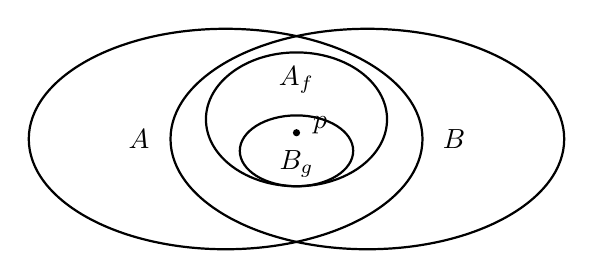
\begin{tikzpicture}[scale=1.0,line width=0.8pt]
    \draw (-0.9,0) ellipse (2.5 and 1.4);
    \draw (0.9,0) ellipse (2.5 and 1.4);
    \node at (-2.0,0) {$\Spec A$};
    \node at (2.0,0) {$\Spec B$};
    \draw (0,0.25) ellipse (1.15 and 0.85);
    \node at (0,0.75) {$\Spec A_f$};
    \draw (0,-0.15) ellipse (0.72 and 0.45);
    \node at (0,-0.32) {$\Spec B_g$};
    \fill (0,0.08) circle (1.3pt);
    \node at (0.30,0.18) {$p$};
  \end{tikzpicture}
  \caption{一个展示「两个仿射开集的交可以被在两个仿射开集中同时特异的开集覆盖」的小技巧。（依原书手绘图重绘。）}\label{fig:affine-communication-trick}
\end{figure}

\emph{证明。}\ （见图~\ref{fig:affine-communication-trick}）任取一点 $p\in\Spec A\cap\Spec B$，我们在 $\Spec A\cap\Spec B$ 中构造 $p$ 的一个开\trNeighborhood，使它同时在 $\Spec A$ 与 $\Spec B$ 中都特异。取 $\Spec A$ 的一个含于 $\Spec A\cap\Spec B$ 且包含 $p$ 的\trDistinguishedOpen{} $\Spec A_f$；再取 $\Spec B$ 的一个含于 $\Spec A_f$ 且包含 $p$ 的\trDistinguishedOpen{} $\Spec B_g$。于是 $g\in\Gamma(\Spec B,\OO_X)$ 限制为一个元素 $g'\in\Gamma(\Spec A_f,\OO_X)=A_f$。$g$ 与 $g'$ 在 $\Spec A_f$ 上消失的点相同，故
\[
\Spec B_g=\Spec A_f\setminus\{[p]\ :\ g'\in p\}=\Spec\bigl(A_f\bigr)_{g'}.
\]
若 $g'=g''/f^n$（其中 $g''\in A$），则 $\Spec(A_f)_{g'}=\Spec A_{fg''}$，证明便告完成。\hfill$\square$

下面这条容易的结果对我们至关重要。

\textbf{5.3.2.\ \trAffineCommunicationLemma。}\ ——\ \emph{设 $P$ 是概形 $X$ 的一些\trAffine\trOpenSubscheme{}所享有的某条性质，使得对 $X$ 的任何\trAffine\trOpenSubscheme{} $\Spec A\hookrightarrow X$：}
\begin{enumerate}[label=(\roman*)]
  \item \emph{若 $\Spec A\hookrightarrow X$ 具有性质 $P$，则对任意 $f\in A$，$\Spec A_f\hookrightarrow X$ 也具有性质 $P$；}
  \item \emph{若 $(f_1,\dots,f_n)=A$（即诸 $\Spec A_{f_i}$ 覆盖 $\Spec A$；参看\cref{ex:distinguished-cover-unit-ideal}），且 $\Spec A_{f_i}\hookrightarrow X$ 对一切 $i$ 都具有 $P$，则 $\Spec A\hookrightarrow X$ 也如此。}
\end{enumerate}
\emph{再设 $X=\bigcup_{i\in I}\Spec A_i$，其中每个 $\Spec A_i$ 都具有性质 $P$。则 $X$ 的每个\trAffine\trOpenSubscheme{}也具有 $P$。}

满足 (i) 与 (ii) 的性质称为\textbf{\trAffineLocal{}}（affine-local）的。这个名称的一个动机是：凭借这条引理，要想判定\emph{每个}\trAffine\trOpenSubscheme{}是否具有该性质，只需在\emph{任何一个}仿射覆盖上检验即可。

举个例子：\trReducedness{}就是一条\trAffineLocal{}的性质。更一般地，任何\trStalkLocal{}的性质（概形具有性质 $P$，当且仅当它的所有\trStalk{}都具有性质 $Q$）必然是\trAffineLocal{}的（概形具有性质 $P$，当且仅当它的所有仿射开集都具有性质 $R$，而仿射概形具有性质 $R$，当且仅当它的所有\trStalk{}都具有性质 $Q$）。但 $Q$ 的正确定义有时并不那么显然；例如可参看下一节关于\trNormality{}的讨论。

\emph{证明。}\ 设 $\Spec A$ 是 $X$ 的一个仿射\trSubscheme{}。用有限多个\trDistinguishedOpen{} $\Spec A_{g_j}$ 覆盖 $\Spec A$，其中每个都在某个 $\Spec A_i$ 中特异。由命题~5.3.1 与 $\Spec A$ 的\trQuasicompactness{}（\cref{ex:spec-quasicompact}(a)），这样做是可行的。由 (i)，每个 $\Spec A_{g_j}$ 都具有 $P$。由 (ii)，$\Spec A$ 具有 $P$。\hfill$\square$

适当地选取性质 $P$，我们便定义出概形的一些重要性质。

\textbf{5.3.3.\ \trhProposition{}。}\ ——\ \emph{设 $A$ 是一个\trRing，且 $(f_1,\dots,f_n)=A$。}
\begin{enumerate}[label=(\alph*)]
  \item \emph{若 $A$ 是\trNoetherian{}环，则每个 $A_{f_i}$ 亦然。若每个 $A_{f_i}$ 都\trNoetherian，则 $A$ 亦然。}
  \item \emph{设 $B$ 是一个\trRing，而 $A$ 是一个 $B$-\trAlgebra（于是对一切 $g\in A$，$A_g$ 都是 $B$-\trAlgebra）。若 $A$ 是\trFinitelyGenerated{}的 $B$-\trAlgebra，则每个 $A_{f_i}$ 亦然。若每个 $A_{f_i}$ 都是\trFinitelyGenerated{}的 $B$-\trAlgebra，则 $A$ 亦然。}
\end{enumerate}

这些断言我们稍后便证（\S5.3.9）。但为了给你一个读证明的动力，我们先\emph{假定}命题~5.3.3 成立，由此给出一些有趣的定义与结果。

\textbf{5.3.4.}\ \emph{重要定义。}\quad 设 $X$ 是一个概形。若 $X$ 能被诸\trAffine\trOpenSet{} $\Spec A$ 覆盖，其中诸 $A$ 都\trNoetherian，就称 $X$ 是一个\textbf{\trLocally\trNoetherian{}\trScheme}（locally Noetherian scheme）。若此外 $X$ 还\trQuasicompact——等价地，能被有限多个这样的\trAffine\trOpenSet{}覆盖——就称 $X$ 是一个\textbf{\trNoetherian{}\trScheme}（Noetherian scheme）。（日后我们会见到许多形如「若 $X$ 具有此性质，就称它为局部 $Q$；若进而 $X$ 还\trQuasicompact，就称它是 $Q$」的定义。）由练习~5.1.C，\trNoetherian{}\trScheme{}的底\trTopologicalSpace{}是\trNoetherian{}的。于是由\cref{ex:noetherian-open-quasicompact}，\trNoetherian{}\trScheme{}的所有\trOpenSubset{}都\trQuasicompact。

\textbf{5.3.A.（练习）}\quad 证明：\trLocally\trNoetherian{}\trScheme{}都是\trQuasiSeparated{}的。

\textbf{5.3.B.（练习）}\quad 证明：\trNoetherian{}\trScheme{}只有有限多个\trIrreducibleComponent。（提示：命题~3.6.15。）证明：\trNoetherian{}\trScheme{}只有有限多个\trConnectedComponent，其中每一个都是有限多个\trIrreducibleComponent{}之并。

\textbf{5.3.C.（练习）}\quad 证明：\trNoetherian{}\trScheme{} $X$ 是\trIntegral{}的，当且仅当 $X$ 非空、\trConnected，且所有\trStalk{} $\OO_{X,p}$ 都是\trIntegralDomain。于是，在「好情形」下，\trIntegrality{}是局部条件（诸\trStalk{}为\trIntegralDomain）与整体条件（\trConnected）二者之并。提示：回想 \trIntegral{}＝\trIrreducible{}＋\trReduced（练习~5.2.G）。若一个概形的诸\trStalk{}都是\trIntegralDomain，则它是\trReduced{}的（\trReducedness{}是一条\trStalkLocal{}条件，定义~5.2.1）。若概形 $X$ 的底\trTopologicalSpace{}是\trNoetherian{}的，则 $X$ 只有有限多个\trIrreducibleComponent{}（由上一练习）；若其中两个在一点 $p$ 相交，则 $\OO_{X,p}$ 不是\trIntegralDomain。（把这件事从\trNoetherian{}\trScheme{}推广到\trLocally\trNoetherian{}\trScheme{}是轻而易举的：只须证明，一个\trConnected{}\trScheme{}是\trIrreducible{}的，当且仅当它非空，且具有一个由开\trIrreducible{}子集构成的\trCover。但某些\trNoetherian{}假设是必要的；参看 [Stacks, tag 0568]。）

\textbf{5.3.5.}\ \emph{不重要的警示。}\quad \trNoetherian{}\trScheme{}的\trGlobalSections{}环未必\trNoetherian；参看练习~19.11.H。

\textbf{5.3.6.\ 给定域 $k$ 之上、或更一般地给定环 $A$ 之上的概形（$A$-\trScheme）。}\quad 你也许特别想在某个特定的域——比如 $\mathbb{C}$ 或 $\mathbb{Q}$——之上工作，或者在诸如 $\mathbb{Z}$ 的环之上工作。受此驱动，我们定义\textbf{$A$-\trScheme}（$A$-scheme）或\textbf{$A$ 上的概形}（scheme over $A$）的概念，其中 $A$ 是一个\trRing：它是一个概形，其\trStructureSheaf{}（在一切\trOpenSet{}上）的诸\trSection{}环都是 $A$-\trAlgebra，并且所有\trRestrictionMap{}都是 $A$-\trAlgebra{}之间的映射。（正如早先诸如\trQuasiseparatedness{}那样的一些观念，这一观念日后将在练习~7.3.I 中被恰当地理解为一个「相对概念」；它的数据是一个\trMorphism{} $X\to\Spec A$。）现在设 $X$ 是一个 $A$-\trScheme。若 $X$ 能被诸\trAffine\trOpenSet{} $\Spec B_i$ 覆盖，且每个 $B_i$ 都是\trFinitelyGenerated{}的 $A$-\trAlgebra，就称 $X$ \textbf{在 $A$ 上\trLocally\trFiniteType}（locally of finite type over $A$），或称它是一个\textbf{\trLocally\trFiniteType{} $A$-\trScheme}（locally finite type $A$-scheme）。（无可否认这套术语颇为累赘；等我们在 \S8.3.9 认识了\trMorphism{}之后，它会更显自然。）若进而 $X$ 还\trQuasicompact，就称 $X$ \textbf{在 $A$ 上\trFiniteType}（finite type over $A$），或称它是一个\textbf{\trFiniteType{} $A$-\trScheme}（finite type $A$-scheme）。注意：在 $k$ 或 $\mathbb{Z}$ 上（或者的确，在任何\trNoetherian{}环上）\trLocally\trFiniteType{}的概形是\trLocally\trNoetherian{}的；类似地，在任何\trNoetherian{}环上\trFiniteType{}的概形是\trNoetherian{}的。作为我们关键的「几何」例子：(i) $\Spec\mathbb{C}[x_1,\dots,x_n]/I$ 是一个\trFiniteType{} $\mathbb{C}$-\trScheme；(ii) $\mathbb{P}^n_{\mathbb{C}}$ 是一个\trFiniteType{} $\mathbb{C}$-\trScheme。（域 $\mathbb{C}$ 可以换成任意\trRing{} $A$。）

\textbf{5.3.D.（练习）}

(a)~（\emph{\trQuasiprojective{}蕴含有限型}）设 $X$ 是一个\trQuasiprojective{} $A$-\trScheme{}（定义~4.5.10），证明 $X$ 在 $A$ 上\trFiniteType。若进而还假定 $A$ \trNoetherian，证明 $X$ 是\trNoetherian{}\trScheme，从而只有有限多个\trIrreducibleComponent。

(b)~设 $U$ 是某射影 $A$-\trScheme{}的一个\trOpenSubscheme。证明 $U$ 在 $A$ 上\trLocally\trFiniteType。若 $A$ \trNoetherian，证明 $U$ \trQuasicompact，从而在 $A$ 上\trQuasiprojective{}，进而由 (a) 在 $A$ 上\trFiniteType。证明当 $A$ 不\trNoetherian{}时这可以不成立。更好的：给出某射影 $A$-\trScheme{}的一个非\trQuasicompact{}\trOpenSubscheme{}的例子（此时 $A$ 必为非\trNoetherian{}的）。（提示：傻例子~4.5.12。）

\textbf{5.3.7.\ \trVariety。}\quad 现在我们来与\trVariety{}的经典语言建立联系。一个既约且在 $k$ 上\trFiniteType{}的\trAffineScheme{}称为一个\textbf{仿射簇}（affine variety (over $k$)），或一个\textbf{仿射 $k$-簇}（affine $k$-variety）。一个既约的（拟）射影 $k$-\trScheme{}是一个\textbf{（拟）射影簇}（(quasi)projective variety (over $k$)），或一个\textbf{（拟）射影 $k$-簇}（(quasi)projective $k$-variety）。（警告：在文献中，簇的定义有时还被额外要求该概形\trIrreducible，或要求 $k$ 是\trAlgClosed{}的。）

\textbf{5.3.E.（练习）}

(a)~证明：$\Spec k[x_1,\dots,x_n]/I$ 是仿射 $k$-簇，当且仅当 $I\subset k[x_1,\dots,x_n]$ 是\trRadicalIdeal。

(b)~设 $I\subset k[x_0,\dots,x_n]$ 是分次的\trRadicalIdeal。证明：$\Proj k[x_0,\dots,x_n]/I$ 是射影 $k$-簇。（警示：例子 $I=(x_0^2,x_0x_1,\dots,x_0x_n)$ 表明，$\Proj k[x_0,\dots,x_n]/I$ 可以是射影 $k$-簇，而 $I$ 却并非根理想。）

我们要到 \S11.2.9 才会在一般情形下定义\trVariety；届时需要先有\trSeparatedness{}的观念，以便排除诸如原点加倍了的仿射直线（例~4.4.5）之类的可憎之物。但本节中我们将要陈述的关于仿射 $k$-簇的许多论断，都会自动适用于更一般的 $k$-簇。

\textbf{5.3.F.（练习）}\quad 证明：\trLocally\trFiniteType{} $k$-\trScheme{}的一点是\trClosedPoint，当且仅当\trStructureSheaf{}在该点处的\trStalk{}的\trResidueField{}是 $k$ 的一个\trFiniteFieldExtension。证明：在\trLocally\trFiniteType{} $k$-\trScheme{}上，诸\trClosedPoint{}是\trDense{}的。提示：\S3.6.9。（警告：即便在相当合理的概形上，\trClosedPoint{}也未必\trDense；参看\cref{ex:closed-points-dense}(b)。）

\textbf{5.3.8.}\ \emph{\trhDefinition{}。}\quad \trLocally\trFiniteType{} $k$-\trScheme{}（例如 $k$ 上的一个\trVariety）中\trClosedPoint{} $p$ 的\textbf{\trClosedPoint{}的\trDegree{}}（degree of a closed point），指的是域扩张 $\kappa(p)/k$ 的\trDegree{}。例如在 $\mathbb{A}^1_k=\Spec k[t]$ 中，点 $[(p(t))]$（其中 $p(t)\in k[t]$ \trIrreducible）的\trDegree{}就是 $\deg p(t)$。若 $k$ 是\trAlgClosed{}的，则每个\trClosedPoint{}的\trDegree{}都是 $1$。

\textbf{5.3.9.}\ \emph{\trhProposition{}~5.3.3 的证明。}\quad 依照\trAffineCommunicationLemma{}~5.3.2 的陈述，我们把每个部分的证明都按 (i) 与 (ii) 分开处理。

\emph{\trhProposition{}~5.3.3(a) 的证明。}\ (i)~设 $\phi:A\to A_f$ 是\trLocalization{}映射。若 $I_1\subsetneq I_2\subsetneq I_3\subsetneq\cdots$ 是 $A_f$ 的\trIdeal{}的一条严格增链，则可以验证 $J_1\subsetneq J_2\subsetneq J_3\subsetneq\cdots$ 是 $A$ 的\trIdeal{}的一条严格增链，其中 $J_i=\phi^{-1}(I_i)$。（我们把 $J_i$ 想成 $I_i\cap A$，只不过一般而言 $A$ 未必\trInjectiveMap{}到 $A_{f_i}$ 中。）显然 $J_i$ 是 $A$ 的\trIdeal。若有 $x/f^n\in I_{i+1}\setminus I_i$，其中 $x\in A$，则 $x\in J_{i+1}$，且 $x\notin J_i$（否则 $x(1/f)^n$ 也将属于 $I_i$）。

(ii)~设 $I_1\subsetneq I_2\subsetneq I_3\subsetneq\cdots$ 是 $A$ 的\trIdeal{}的一条严格增链。则对每个 $1\le i\le n$，
\[
I_{i,1}\subset I_{i,2}\subset I_{i,3}\subset\cdots
\]
是 $A_{f_i}$ 中\trIdeal{}的一条增链，其中 $I_{i,j}=I_j\otimes_A A_{f_i}$。尚须证明：对每个 $j$，存在某个 $i$ 使 $I_{i,j}\subsetneq I_{i,j+1}$；届时结论即随之而来。

\textbf{5.3.G.（练习）}\quad 完成命题~5.3.3(a) 的证明。（提示：若 $M:=I_j/I_{j-1}\neq0$，则由 $M\hookrightarrow\prod_i M_{f_i}$（\eqref{eq:module-equalizer-sequence}），某个 $M_{f_i}$ 非零。）

\emph{\trhProposition{}~5.3.3(b) 的证明。}\ 部分 (i) 是显然的：若 $A$ 由 $r_1$、……、$r_n$ 在 $B$ 上生成，则 $A_f$ 由 $r_1$、……、$r_n$、$1/f$ 在 $B$ 上生成。

(ii)~思路如下。由于诸 $f_i$ 生成 $A$，我们可以写出 $1=\sum c_if_i$，其中 $c_i\in A$。我们有诸 $A_{f_i}$ 的生成元：$r_{ij}/f_i^{k_i}$，其中 $r_{ij}\in A$。我断言：$\{f_i\}_i\cup\{c_i\}\cup\{r_{ij}\}_{ij}$ 作为 $B$-代数生成 $A$。理由如下。任取 $r\in A$。在 $A_{f_i}$ 中，我们可以把 $r$ 写成关于诸 $r_{ij}$ 与 $f_i$ 的某个多项式除以 $f_i$ 的某次巨大的幂。于是「在每个 $A_{f_i}$ 中，我们都已按要求描述了 $r$」，只差这枚烦人的分母。现在沿用\cref{thm:sheaf-on-distinguished-base}证明中那类「\trPartitionOfUnity{}」式的论证，把所有这些拼成一个单一的表达式，杀掉分母。证明你造出的表达式在每个 $A_{f_i}$ 中仍与 $r$ 一致。于是它确实就是 $r$（依据\trStructureSheaf{}的\trIdentityAxiom）。

\textbf{5.3.H.（练习）}\quad 把这个论证精确化。

至此，命题~5.3.3 的证明便告完成。\hfill$\square$
